%%%%%%%%%%%%%%%%%%%%%%%%%%%%%%%%%
% baposter Landscape Poster
% LaTeX Template
% Version 1.0 (15/5/13)
%
% Created by:
% Brian Amberg (baposter@brian-amberg.de)
%
% This template has been downloaded from:
% http://www.LaTeXTemplates.com
%
% License:
% CC BY-NC-SA 3.0 (http://creativecommons.org/licenses/by-nc-sa/3.0/)
%
%%%%%%%%%%%%%%%%%%%%%%%%%%%%%%%%%%%%%%%%%

%----------------------------------------------------------------------------------------
%	PACKAGES AND OTHER DOCUMENT CONFIGURATIONS
%----------------------------------------------------------------------------------------

\documentclass[a0paper,portrait,fontscale=0.355, margin=2cm]{baposter}

\usepackage[utf8]{inputenc}
\usepackage[font=normalsize,labelfont=bf]{caption} % Required for specifying captions to tables and figures
\captionsetup{justification=centering}
\usepackage{booktabs} % Horizontal rules in tables
\usepackage{lmodern}
\usepackage{relsize} % Used for making text smaller in some places

% Other packages
\usepackage{tabularx}
\def\tabularxcolumn#1{m{#1}}
\def\imagetop#1{\vtop{\null\hbox{#1}}}
\usepackage{adjustbox}
\usepackage{subfig}
\usepackage{floatrow} % sidecapfloat
\usepackage{setspace}
\usepackage{xspace}
\usepackage{noReferences}
\usepackage{caption}
\usepackage{tikz}
\usepackage[customcolors]{hf-tikz}
%\usepackage{subcaption}
\usepackage{epsf}
\usepackage{amsmath}
\usepackage{mathtools}
\usepackage{amssymb}
\usepackage{amsfonts}
\usepackage{amsthm}
\usepackage{dsfont}
\usepackage{enumitem}
\usepackage{float}
\usepackage{cases}
\usepackage{verbatim}
\usepackage{array}
\usepackage{graphicx}
\usepackage{graphics}
\usepackage{multirow}
\usepackage{listings}
%\usepackage[authoryear]{natbib}
\usepackage{authblk}
\usepackage[linesnumbered,ruled,vlined]{algorithm2e}
\usepackage{eqparbox}
\usepackage{xcolor}
\usepackage[backend=biber, citestyle=authoryear, maxcitenames=2, maxbibnames=2]{biblatex}
\usepackage{lipsum}
\usepackage{svg}
\usepackage{cleveref}

\bibliography{../budgeted_rl.bib}

\input{style}
\input{../mathdef}


\begin{document}


%\background{ % Set the background to an image (background.pdf)
%\begin{tikzpicture}[remember picture,overlay]
%\draw (current page.north west)+(-2em,2em) node[anchor=north west]
%{\includegraphics[height=1.1\textheight]{background.png}};
%\end{tikzpicture}
%}
\begin{poster}{
grid=false,
borderColor=bordercol, % Border color of content boxes
headerColorOne=headercol1, % Background color for the header in the content boxes (left side)
headerColorTwo=headercol2, % Background color for the header in the content boxes (right side)
headerFontColor=headerfontcol, % Text color for the header text in the content boxes
boxColorOne=boxcolor, % Background color for the content in the content boxes
headershape=roundedright, % Specify the rounded corner in the content box headers
%headerfont=\Large\sf\bf, % Font modifiers for the text in the content box headers
headerfont=\Large\bf\textsc, %Sans Serif
textborder=rectangle,
background=none,
headerborder=open, % Change to closed for a line under the content box headers
boxshade=plain,
textfont={\setlength{\parindent}{0.0em}\sffamily},
headerheight={0.05\textheight},
eyecatcher=true
%columns=5
}
%
%----------------------------------------------------------------------------------------
%	Title and authors
%----------------------------------------------------------------------------------------
%
{
\includegraphics[width=18em]{./img/companies}
}
{
Budgeted Reinforcement Learning in Continuous State Space
}
{
Nicolas Carrara, Edouard Leurent, Romain Laroche, \\Tanguy Urvoy, Odalric-Ambrym Maillard, Olivier Pietquin
\vspace{-3\baselineskip}
}
{
\includegraphics[width=14em]{./img/inria_sc}
}

\setlength{\colheight}{0.92\textheight}

%----------------------------------------------------------------------------------------
%	Motivation
%----------------------------------------------------------------------------------------

\headerbox{\textsc{Motivation}}{name=motivation,span=1,column=0,row=0}{

\textbf{Markov Decision Process} $(\cS, \cA, P, R_r, \gamma)$:
\begin{equation*}
    \max_\pi \expectedvalue_\pi \underbrace{\sum_{t=0}^\infty \gamma^t R_r(s_t, a_t)}_{G_r^\pi}
\end{equation*}

\begin{itemize}[nolistsep]
    \item[\incarrow] \hlr{Single scalar reward} to represent \hlr{multiple} \hlr{contradictory} aspects (e.g. complete task and avoid collisions)
    \item[\incarrow] \hlr{No control over the spread} of the performance distribution\\
     
\end{itemize}

\textbf{Constrained MDP} $(\cS, \cA, P, R_r, R_c, \gamma)$
\begin{itemize}[nolistsep]
    \item $[$\cite{BEUTLER1985236,Altman95constrainedmarkov}$]$
    \item Introduce a \hlb{cost signal} $R_c$
    \item Constrained objective
\begin{equation*}
\begin{array}{lcr}
 \displaystyle \max_{\pi\in\cM(\cA)^\cS} \expectedvalue[G_r^\pi | s_0=s] & \text{\hlb{ s.t. }} & \expectedvalue[G_c^\pi | s_0=s] \leq \beta
\end{array}
\end{equation*}
\item[\incarrow] The cost budget $\beta$ \hlr{cannot be changed} after training\\
\end{itemize}

\textbf{Budgeted MDP}

\begin{itemize}[nolistsep]
    \item $[$\cite{Boutilier_Lu:uai16}$]$
    \item We seek \hlg{one general policy} $\pi(s,\beta)$ that solves every CMDP for any $\beta$
    \item[\incarrow] Can only be solved for \hlr{finite} $\cS$ and \hlr{known} $P, R_r, R_c$.
\end{itemize}
}

%----------------------------------------------------------------------------------------
%	Setting
%----------------------------------------------------------------------------------------
\headerbox{\textsc{Setting}}{name=setting,span=1,column=0,row=0,below=motivation}{

\textbf{Budgeted policies} $\pi$
\begin{itemize}
    \item Take a budget $\beta$ as an additional input
    \item Output a next budget $\beta'$ 
\end{itemize}
\begin{equation*}
    \pi:\underbrace{(s,\beta)}_{\os} \rightarrow \underbrace{(a,\beta')}_{\oa}
\end{equation*}

\textbf{2D  signals}
\begin{enumerate}
    \item Rewards $R = (R_r, R_c)$
    \item Returns $G^\pi = (G_r^\pi, G_c^\pi)$
    \item Values $V^\pi = (V_r^\pi, V_c^\pi)$ and $Q^\pi = (Q_r^\pi, Q_c^\pi)$\\
\end{enumerate}

\textbf{Policy Evaluation}\\

The Bellman Expectation equations% [\cite{Bellman}]
are preserved, and the Bellman Expectation Operator $\cT^\pi$ is a \hlg{$\gamma$-contraction}.
}

%----------------------------------------------------------------------------------------
%	Budgeted Optimality
%----------------------------------------------------------------------------------------
\headerbox{Budgeted Optimality}{name=bopt,column=0,span=1,below=setting}{
\begin{definition*}In that order, we want to:
\begin{enumerate}
    \item[(i)] \hlb{Respect the budget $\beta$}: 
    \begin{equation*}
    \Pi_a(\os) \eqdef \{\pi\in\Pi: V_c^\pi(s, \beta) \leq \beta\}
    \end{equation*}
    \item[(ii)] \hlg{Maximise the rewards}:
    \begin{equation*}
        V_r^*(\os) \eqdef {\max}_{\pi\in\Pi_a(\os)}  V_r^\pi(\os) \qquad\quad \Pi_r(\os) \eqdef \argmax_{\pi\in\Pi_a(\os)}  V_r^\pi(\os)
    \end{equation*}
    \item[(iii)] \hlr{Minimise the costs}: 
    \begin{equation*}
        V_c^*(\os) \eqdef {\min}_{\pi\in\Pi_r(\os)}  V_c^\pi(\os), \qquad\quad \Pi^*(\os) \eqdef \argmin_{\pi\in\Pi_r(\os)}  V_c^\pi(\os)
    \end{equation*}
\end{enumerate}

We define the budgeted action-value function $Q^*$ similarly
\end{definition*}

}

%----------------------------------------------------------------------------------------
%	Budgeted Dynamic Programming
%----------------------------------------------------------------------------------------
\headerbox{Budgeted Dynamic Programming}{name=bdp,column=1,span=2}{

\begin{minipage}{0.7\textwidth}
\bookboxx{
\begin{theorem*}[Budgeted Bellman Optimality]
\label{thm:bellman-optimality}
$Q^*$ verifies:
\begin{equation}
\label{eq:bellman-optimality}
    \hleb{\vphantom{\frac{A}{A}} Q^{*}(\os, \oa) = \cT Q^{*}(\os, \oa)}  \eqdef R(\os, \oa) + \gamma \sum_{\os'\in\ocS} \ov{P}(\ov{s'} | \os, \oa)\sum_{\ov{a'}\in \ocA} \pi_\text{greedy}(\ov{a'}|\ov{s'}; Q^*) Q^{*}(\ov{s'}, \ov{a'}),
\end{equation}
where the greedy policy $\pi_\text{greedy}$ is defined by:
\begin{subequations}
\label{eq:pi_greedy}
\begin{align}
    \pi_\text{greedy}(\oa|\os; Q) \in &\hler{\argmin}_{\rho\in\Pi_r^Q} \expectedvalueover{\oa\sim\rho}Q_c(\os, \oa), \label{eq:pi_greedy_cost}\\
    \text{where }\quad\Pi_r^Q \eqdef &\hleg{\argmax}_{\rho\in\cM(\ocA)} \expectedvalueover{\oa\sim\rho} Q_r(\os, \oa) \label{eq:pi_greedy_reward}\\
    & \text{ s.t. }  \expectedvalueover{\oa\sim\rho} Q_c(\os, \oa) \hleb{\leq \beta} \label{eq:pi_greedy_constraint}
\end{align}
\end{subequations}
\end{theorem*}
}
\bookboxx{
\begin{proposition*}
\label{prop:greedy_optimal}
$\pi_\text{greedy}(\cdot~; Q^*)$ is \hlg{simultaneously optimal} in all states $\os\in\ocS$: $$\pi_\text{greedy}(\cdot~; Q^*)\in\Pi^*(\os)$$

In particular, $V^{\pi_\text{greedy}(\cdot; Q^*)} = V^*$ and $Q^{\pi_\text{greedy}(\cdot; Q^*)}= Q^*$.
\end{proposition*}
}

\end{minipage}
\hfill%
\begin{minipage}{0.25\textwidth}
\begin{algorithm}[H]
\DontPrintSemicolon
\KwData{$P, R_r, R_c$}
\KwResult{$Q^*$}
$Q_{0} \leftarrow 0$\;
\Repeat{convergence}{
    $Q_{k+1} \leftarrow \cT Q_k$\;
}
\caption{Budgeted Value Iteration}
\label{algo:bvi}
\end{algorithm}
\begin{center}
\includegraphics[width=0.9\textwidth]{source/img/concavity_example.pdf}    
\end{center}
\end{minipage}

\bookboxx{
\begin{theorem*}[Contractivity]
\label{thm:contraction}
For any BMDP ($\cS,\cA,P,R_r,R_c,\gamma$) with $|\cA| \geq 2$, \hlr{$\cT$ is not a contraction}. 
$$\forall\epsilon>0, \exists Q^1,Q^2\in(\Real^2)^{\ocS\ocA}:\|\cT Q^1-\cT Q^2\|_\infty \geq \frac{1}{\epsilon}\|Q^1-Q^2\|_\infty$$
\end{theorem*}
}

Despite those theoretical limitations, we observed \hlg{empirical convergence} in our experiments

\bookboxx{
\begin{remark*}[Contractivity on smooth $Q$-functions]
\label{rmk:contractivity-smooth}
We conjecture that \hlg{$\cT$ is a contraction when restricted} to the subset $\cL_\gamma$ of $Q$-functions such that "$Q_r$ is \hlg{$L$-Lipschitz} with respect to $Q_c$", with $L<\frac{1}{\gamma}-1$.
\end{remark*}
}
}

%----------------------------------------------------------------------------------------
%	Budgeted Reinforcement Learning
%----------------------------------------------------------------------------------------
\headerbox{Budgeted Reinforcement Learning}
{name=brl,span=2,column=1,below=bdp}{ 

We address several limitations of \Cref{algo:bvi}.\\

\begin{minipage}{0.65\textwidth}
\begin{enumerate}
    \item The BMDP is \hlr{unknown}
\begin{itemize}[nolistsep]
    \item[\incarrow] Work with a \hlg{batch} of samples $\cD=\{(\os_i,\oa_i,r_i,\os_i'\}_{i\in [0,N]}$
\end{itemize}
\item $\cT$ contains an \hlr{expectation} $\expectedvalue_{\os'\sim \ov{P}}$ over next states $\os'$
\begin{itemize}[nolistsep]
    \item[\incarrow] Replace it with a \hlg{sampling} operator $\hat{\cT}$:
\begin{equation*}
    \hat{\cT} Q(\os_i, \oa_i, r_i, \os'_i) \eqdef r_i + \gamma \sum_{\ov{a'_i}\in \cA_i} \pi_\text{greedy}(\ov{a'_i}|\ov{s'_i}; Q) Q(\ov{s'_i}, \ov{a'_i}).
\end{equation*}
\end{itemize}
\item $\cS$ is \hlr{continuous}
\begin{itemize}[nolistsep]
    \item[\incarrow] Employ \hlg{function approximation} $Q_\theta$, and minimise a regression loss 
    $$\cL(Q_\theta, Q_\text{target};\cD) = \sum_{\cD} ||Q_\theta(\os, \oa) - Q_\text{target}(\os, \oa, r, \os')||_2^2$$
\end{itemize}
\end{enumerate}

\end{minipage}
\begin{minipage}{0.34\textwidth}
\begin{algorithm}[H]
\DontPrintSemicolon
\KwData{$\cD$}
\KwResult{$Q^*$}
$Q_{\theta_0} \leftarrow 0$\;
\Repeat{convergence}{
    $\theta_{k+1} \leftarrow \argmin_\theta \cL(Q_\theta, \hat{\cT} Q_{\theta_{k}}; \cD)$\;
}
\caption{Budgeted Fitted-Q Iteration}
\label{algo:bftq}
\end{algorithm}
\vspace{1em}
\begin{enumerate}[nolistsep]
    \item[4.] How to \hlr{collect the batch} $\cD$?
    \begin{itemize}[nolistsep]
        \item[\incarrow] We propose a \hlg{risk-sensitive} exploration procedure
    \end{itemize}
\end{enumerate}
\end{minipage}
}

%----------------------------------------------------------------------------------------
%	Scalable Implementation
%----------------------------------------------------------------------------------------
\headerbox{Scalable Implementation}{name=scale,span=2,column=1,below=brl}{ 

\begin{minipage}[t]{0.48\textwidth}
\textbf{How to compute the greedy policy?}

\begin{center}
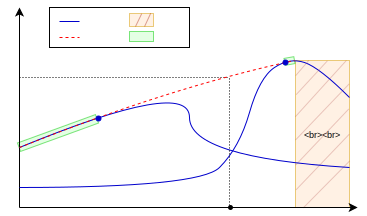
\includegraphics[width=0.8\linewidth]{../source/img/pi.pdf}    
\end{center}
\vspace*{-1em}
\bookboxx{
\begin{proposition*}[Hull policy]
\label{prop:bftq_pi_hull}
$\pi_\text{greedy}$ in \eqref{eq:pi_greedy} can be \hlg{computed explicitly}, as a mixture of two points that lie on the convex hull of $Q$.
\end{proposition*}
}

\end{minipage}
\hfill%
\begin{minipage}[t]{0.48\textwidth}

\textbf{Function approximation}

\begin{center}
\resizebox{.7\textwidth}{!}{%
\input{../source/architecture.tex}
}    
\end{center}


\textbf{Parallel computing}

Experience collection and computation of $\pi_\text{greedy}$ can be distributed over several cores.

\end{minipage}
}

%
%%----------------------------------------------------------------------------------------
%% Experiments
%%----------------------------------------------------------------------------------------
%
\headerbox{Experiments}{name=experiments,span=2,column=1,below=scale, above=bottom}{ 

\begin{minipage}{0.49\textwidth}
\centering
Risk-sensitive exploration

\includegraphics[width=0.3\textwidth]{source/img/test.pdf}
\includegraphics[page=1, width=0.49\textwidth]{source/img/corridors}
\end{minipage}
\begin{minipage}{0.5\textwidth}
\centering
Pareto frontier

\includegraphics[width=0.49\linewidth]{../source/img/slot-filling}
\includegraphics[width=0.49\linewidth]{../source/img/highway}
\end{minipage}
}



%----------------------------------------------------------------------------------------
%	Acknowledgements
%----------------------------------------------------------------------------------------
\headerbox{Acknowledgements}{name=ack,column=0,span=1,below=bopt}{
This work has been supported by CPER Nord-Pas de Calais/FEDER DATA Advanced data science and technologies 2015-2020, the French Ministry of Higher Education and Research, INRIA, and the French Agence Nationale de la Recherche (ANR).
}


%----------------------------------------------------------------------------------------
%	References
%----------------------------------------------------------------------------------------
\headerbox{References}{name=refs,column=0,span=1,below=ack, above=bottom}{
    {
    \AtNextBibliography{\footnotesize}
    \setlength{\bibitemsep}{3pt}
    \printbibliography[heading=none]
    }
}


\end{poster}

\end{document}


